% Rotor: camino cerrado para la circulación (libro fig. 2.9)
\documentclass[border=5pt]{standalone}
\usepackage{tikz}
\usetikzlibrary{arrows.meta}
\begin{document}
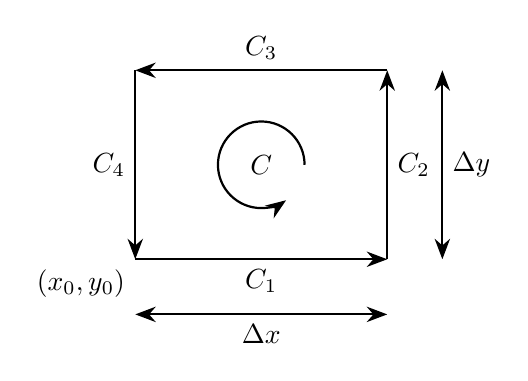
\begin{tikzpicture}[>={Stealth[length=2.6mm]}, line width=0.8pt]
  \coordinate (BL) at (0,0);
  \coordinate (BR) at (3.2,0);
  \coordinate (TR) at (3.2,2.4);
  \coordinate (TL) at (0,2.4);
  \draw[->] (BL)--(BR); \node[below] at (1.6,0){$C_1$};
  \draw[->] (BR)--(TR); \node[right] at (3.2,1.2){$C_2$};
  \draw[->] (TR)--(TL); \node[above] at (1.6,2.4){$C_3$};
  \draw[->] (TL)--(BL); \node[left] at (0,1.2){$C_4$};
  \node[below left] at (BL){$(x_0,y_0)$};
  % circulación central
  \draw[->] (1.6,1.2)+(0.55,0) arc (0:305:0.55);
  \node at (1.6,1.2){$C$};
  % dimensiones
  \draw[<->] (0,-0.7)--(3.2,-0.7) node[midway,below]{$\Delta x$};
  \draw[<->] (3.9,0)--(3.9,2.4) node[midway,right]{$\Delta y$};
\end{tikzpicture}
\end{document}
